\section{はじめに}
%
%%% GOAL
%
\subsection{課題 1 の目標とテーマ}
\begin{frame}
\frametitle{課題 1の目標とテーマ}
  \begin{columns}
    \begin{column}{0.6\textwidth}
      \begin{itemize}
\item 目標
        \begin{itemize}
\item 計算の基本要素を知る
        \end{itemize}
\item テーマ
        \begin{itemize}
\item 四則演算でアニメーション
\item \movie[once,externalviewer]{\beamerbutton{ひつじさん}}{./Figure/sheep-python.mov}
        \end{itemize}
      \end{itemize}
    \end{column}
    \begin{column}{0.4\textwidth}
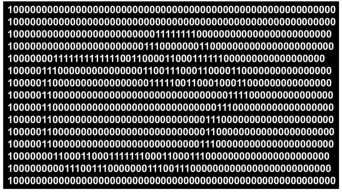
\includegraphics[scale=0.6]{./Figure/sheep-fixed.pdf}
    \end{column}
  \end{columns}
\end{frame}
\subsection{CS のこころ}
\begin{frame}
\frametitle{CS のこころ}
  \begin{itemize}
\item しつこいようですが,すべては計算
\item コンピュータに載せるには
    \begin{itemize}
\item 対象をデータとして表すこと
\item 処理を基本演算の組み合わせで表すこと
    \end{itemize}
\item 処理とはコンピュータのなかの抽象的な世界に存在して
\item データというもう一つの抽象的な存在を操作する
\item この処理やデータをプログラミング言語の記号をもちいて注意深く構成したのがプログラム
  \end{itemize}
\end{frame}
%
%%% What's DATA
%
\section{データは数である}
\begin{frame}
\frametitle{データは数である}
  \begin{itemize}
\item データから見ていくことにして
\item データはすべて 2 進列で表される
    \begin{itemize}
\item 自然数,整数,実数: 18, -3, 3.14 など
\item 文字: 文字コード: ASCII, Unicode など
\item 画像,映像
\item 音
\item におい,味,触覚
    \end{itemize}
  \end{itemize}
\end{frame}
%
%%% Number
%
\subsection{Bit と Byte}
\begin{frame}
\frametitle{情報とは}
  \begin{itemize}
\item ここで情報とは何か考えてみます
\item 情報とは"ある物事,事情についてのお知らせ"
\item 情報の価値はどう決まるか?
    \begin{itemize}
\item 驚きをもって受け止められる情報は価値が高い?
\item 日常的な情報は価値が低い?
    \end{itemize}
  \end{itemize}
\end{frame}
\begin{frame}
\frametitle{まずは情報量というもの}
  \begin{enumerate}
\item ある結果や情報を得る場合を考える
\item 結果や情報を生じる事象が確率現象であると見なす
\item 確率 $p$ の事象の情報量を \(I(p)\) であらわす
\item \(I(p)\) は単調減少関数
    \begin{itemize}
\item 頻繁に起こっていること ((\(p\) が大きい) は情報量が少ない)
\item 頻繁に起こらないこと ((\(p\) が小さい) は情報量が多い)
    \end{itemize}
\item 連続関数である
    \begin{itemize}
\item 確率のわずかな変化で情報量が大きく変化するのは不自然
    \end{itemize}
  \end{enumerate}
  \begin{block}{情報量の定義}
ある事象 $a$ の生起確率を \(p_a\) とすると
その情報量 \(I(p_a)\) は \(\log_{2}\frac{1}{p_a}=-\log_{2}p_a\) であらわすことにする
  \end{block}
\end{frame}
\begin{frame}
\frametitle{ビットとは}
  \begin{block}{1 bit とは}
    \begin{enumerate}
\item 今, 2 つの事象を考える
\item 同じ確率 \(P=\frac{1}{2}\) で生起するとする
\item このとき,ひとつの事象 $a$ の情報量 \(I(a)=\log_2\frac{1}{\frac{1}{2}}=1\)
\item これが 1 bit
\item 確率 \(\frac{1}{2}\) で起こる事象を知った時の情報量が 1 bit(ビット)
    \end{enumerate}
  \end{block}
  \begin{itemize}
\item それでは確率 \(\frac{1}{10}\) で起こる事象を知った時は 1 hartley(ハートレー)
\item 確率 \(\frac{1}{e}\) では 1 nat(ナット)
  \end{itemize}
\end{frame}
\begin{frame}
\frametitle{情報の記録}
  \begin{itemize}
\item 情報はビットの列として記録
\item 明確に区別された 2 つの状態で記録しています
    \begin{itemize}
\item 磁性体の向き,電圧の高低,スイッチの開閉
    \end{itemize}
\item 計算機科学では 2 つの状態を便宜的に $0$ と $1$ として議論しています
  \end{itemize}
\end{frame}
\begin{frame}
\frametitle{ビットによる表現}
  \begin{itemize}
\item 2 つの状態を取り得るデバイスを $N$ 個並べてそれぞれ独立としたらどれだけの情報があらわせるか
\item 答えは \(\log_2 2^N=N\) となり $N$ ビットの情報量となります
\item $N$ ビットでどれだけの事象を区別できるでしょうか
\item 答えは 2 個の要素から $N$ 個の重複順列 \({ }_2\Pi_N=2^N\) です
  \end{itemize}
\end{frame}
\begin{frame}
\frametitle{バイトとは}
  \begin{itemize}
\item 人間にとって意味をなす長さ $N$ の小ブロック
\item 現在のコンピュータでは 8 bit としています
  \end{itemize}
\end{frame}
%
%%% Number
%
\subsection{自然数の n 進表記}
\begin{frame}
\frametitle{数表記}
  \begin{itemize}
\item ビットの列で表すことは先に述べました
\item では自然数はどうあらわすでしょう
\item 数表記は 10 進が唯一の方法ではありません
\item $n$ 進表記が可能です
\item 数はどうコンピュータ内で表現されるかみていきます
  \end{itemize}
\end{frame}
\begin{frame}
\frametitle{$n$ 進表記}
  \begin{itemize}
\item 実は日常的に $n$ 進法を利用しています
\item 時間は 24 進法, 60 進法, 30 進法,360 進法をもちいています
\item たとえば 24 進法では 24 になったら位が一つ上がります
\item コンピュータでは 2 進法をもちいて自然数を表します
\item 2 進法ではやはり人間には分かりずらいので 8 進法や 16 進法であらわすことが多いです
  \end{itemize}
\end{frame}
\begin{frame}
\frametitle{$n$ 進法の各桁}
  \begin{itemize}
\item 2 進法,8 進法,16 進法でも 10 進法と同じように位どりによってあらわします
\item 良くご存知のように 10 進法では 1 桁を 0-9 のいづれかであらわしています
\item 123 という自然数であれば \(1\times 10^2+2\times 10^1+3\times 10^0\) といった具合です
  \end{itemize}
\end{frame}
\begin{frame}
\frametitle{2 進法の各桁}
  \begin{itemize}
\item 2 進法では各桁は 0 と 1 だけになります
\item 10 進法の場合と同様に位どりします,ただし底が 2 になります
\item \((010)_2\) という自然数であれば \(0\times 2^2+1\times 2^1+0\times 2^0\) といった具合です
\item この例では \((2)_{10}\) は位が一つ上がって \((010)_2\) となっています
  \end{itemize}
\end{frame}
\begin{frame}
\frametitle{16 進法の各桁}
  \begin{itemize}
\item 2 進法では桁が多くなって見ずらいので 16 進で表記します
\item 16 進法では各桁:
    \begin{itemize}
\item 0,1,2,3,4,5,6,7,8,9 と 0-9 までは 10 進と同じ
\item 10,11,12,13,14,15 は A,B,C,D,E,F をもちいます
    \end{itemize}
\item 10 進法の場合と同様に位どりします,ただし底が 16 になります
\item \((1F0)_{16}\) という自然数であれば \(1\times 16^2+F\times 16^1+0\times 16^0\) といった具合です
  \end{itemize}
\end{frame}
\begin{frame}
\frametitle{各数字の対応}
  \begin{columns}[t]
    \begin{column}{5cm}
\footnotesize
      \begin{tabular}{c|c|c|c}
10 進 & 8 進 & 16 進 & 2 進\\
\hline
 0& 0& 0&0\\
 1& 1& 1&1\\
 2& 2& 2&10\\
 3& 3& 3&11\\
 4& 4& 4&100\\
 5& 5& 5&101\\
 6& 6& 6&110\\
 7& 7& 7&111\\
      \end{tabular}
    \end{column}
    \begin{column}{5cm}
\footnotesize
      \begin{tabular}{c|c|c|c}
10 進 & 8 進 & 16 進 & 2 進\\
\hline
 8&10& 8&1000\\
 9&11& 9&1001\\
10&12& A&1010\\
11&13& B&1011\\
12&14& C&1100\\
13&15& D&1101\\
14&16& E&1110\\
15&17& F&1111\\
      \end{tabular}
    \end{column}
  \end{columns}
\end{frame}
\begin{frame}[label=Dec2Bin]
\frametitle{$n$ 進数の変換}
  \begin{itemize}
\item $m$ 進数から $n$ 進数への変換
\item 手始めに 10 進数から 2 進数への変換
  \end{itemize}
  \begin{center}
   \begin{example}[10進$\Leftrightarrow$2進]
   \begin{columns}[t]
    \begin{column}{3cm}
\infer[\mbox{High}]{0}{\infer{2)1\cdots 1}{\infer{2)2\cdots 0}{\infer{2)4\cdots 0}{\infer[\mbox{Low}]{2)9\cdots 1}{2)19\cdots 1}}}}}
    \end{column}
    \begin{column}{3cm}
\infer{19}{\infer{1\times 2^4=16}{\infer{0\times 2^3=0}{\infer{0\times 2^2=0}{\infer{1\times 2^1=2}{1\times 2^0=1}}}}}
    \end{column}
   \end{columns}
   \end{example}
  \end{center}
\end{frame}
\begin{frame}
\frametitle{Quiz: 10 進表記$\Leftrightarrow$ 2 進表記 の変換}
  \begin{block}{Quiz}
    \begin{enumerate}
\item 131$_{10}$, 112$_{10}$ を 2 進数に変換してみてください\label{lb:first}
\item \ref{lb:first}で得られた 2 進数を 10 進表記に戻してください
\item もとの 10 進数が得られれば正しく変換できています
\item この数字は東工大に割り当てられた IP アドレスになります
    \end{enumerate}
  \end{block}
\end{frame}
%\section{数の表現}
\begin{frame}[shrink]
\frametitle{繰り返しや再帰によるその他の計算}
  \begin{itemize}
\item 繰り返しや再帰は自然数 $n$ に対応する解を求めるような感じ
    \begin{itemize}
\item 数列は $n$ 番目の数を求める: \(\alpha\colon N\rightarrow N\)
\item ハノイの塔も $n$ 枚目の解を求める
    \end{itemize}
\item これを利用して関数の解を求める計算に利用する
\item たとえば非線形方程式 \(f(x)=0\) の実根を求める
\item \href{run:newton.command}{\beamerbutton{ニュートン法}}
    \begin{itemize}
\item \(\sqrt{a}\) を求めてみる
\item \(f(x)=x^2-a\) として \(f(x)=0\) となる $x$ を求める
\item \(k+1\) 番目の近似値 \(x_{k+1}\) を
      \begin{displaymath}
x_{k+1} = x_k-\frac{f(x_k)}{f'(x_k)} = \frac{1}{2}(x_k+\frac{a}{x_k})
      \end{displaymath}
で求める
\item \(x_{k+1}\) と \(x_k\) が十分近くなったら停止
    \end{itemize}
  \end{itemize}
\end{frame}
\subsection{非負整数の表現}
\begin{frame}[label=Top_Integer]
\frametitle{非負整数のコンピュータ内での表現}
  \begin{itemize}
\item 10 進数から 2 進数への変換
  \end{itemize}
  \begin{center}
   \begin{example}[10進$\Leftrightarrow$2進]
   \begin{columns}[t]
    \begin{column}{3cm}
\infer[\mbox{High}]{0}{\infer{2)1\cdots 1}{\infer{2)2\cdots 0}{\infer{2)4\cdots 0}{\infer[\mbox{Low}]{2)9\cdots 1}{2)19\cdots 1}}}}}
    \end{column}
    \begin{column}{3cm}
\infer{19}{\infer{1\times 2^4=16}{\infer{0\times 2^3=0}{\infer{0\times 2^2=0}{\infer{1\times 2^1=2}{1\times 2^0=1}}}}}
    \end{column}
   \end{columns}
   \end{example}
  \end{center}
\end{frame}
\subsection{負の数の表現}
\begin{frame}[shrink]
\frametitle{負の数の表現}
  \begin{itemize}
\item 負の数をあらわすには補数表現をもちいます
\item それでは 2 の補数(2's complement) を求めてみましょう
  \end{itemize}
  \begin{block}{2 の補数表現}
    \begin{enumerate}
\item 2 進表記において各ビットを反転する
\item それに 1 を足す
    \end{enumerate}
  \end{block}
  \begin{center}
    \begin{example}[-8$\sim$7 (2 進 4 桁) の 2 の補数表現]
\((1000)_{(2)}\Rightarrow(1001)_{(2)}\Rightarrow(1010)_{(2)}\Rightarrow (1011)_{(2)}\Rightarrow (1100)_{(2)}
\Rightarrow(1101)_{(2)}\Rightarrow(1110)_{(2)}\Rightarrow(1111)_{(2)}
\Rightarrow(0000)_{(2)}\Rightarrow(0001)_{(2)}\Rightarrow(0010)_{(2)}\Rightarrow(0011)_{(2)}
\Rightarrow(0100)_{(2)}\Rightarrow(0101)_{(2)}\Rightarrow(0110)_{(2)}\Rightarrow(0111)_{(2)}\)\\
      \begin{itemize}
\item Successor (1 足す) でつぎの数になるようになっている
\item 最上位ビットがサインビットになっている
\item circulation の実行
      \end{itemize}
    \end{example}
  \end{center}
\end{frame}
\subsection{計算機内の計算}
\begin{frame}[shrink]
\frametitle{計算機内の計算}
\framesubtitle{整数の減算}
  \begin{itemize}
\item 2 進 $n$ 桁の数 $a, b$ (\(A_k,B_k\in\{1,0\}\))
    \begin{itemize}
\item \(a\colon A_{n-1}A_{n-2}\cdots A_{1}A_{0}\)
\item \(b\colon B_{n-1}B_{n-2}\cdots B_{1}B_{0}\)
    \end{itemize}
\item \(a, b\) はそれぞれ
\[a=\sum_{k=0}^{n-1}2^{k}A_{k}\]
\[b=\sum_{k=0}^{n-1}2^{k}B_{k}\]
\item $b$ の各桁を反転させたものを \(\overline{B_{k}}\) として $b$ の補数 \(\overline{b}\) は
\[\overline{b}=\sum_{k=0}^{n-1}2^{k}\overline{B_{k}}=\sum_{k=0}^{n-1}2^{k}(1-B_{k})=(2^n-1)-b\]
  \end{itemize}
\end{frame}
\begin{frame}[shrink]
\frametitle{計算機内の計算\textemdash Cont.}
  \begin{itemize}
\item \(\overline{b}=(2^n-1)-b\) より
    \begin{eqnarray*}
a-b&\Rightarrow& a-((2^n-1)-\overline{b})\\
   &=&a+\overline{b}+1-2^n
    \end{eqnarray*}
\item 引き算は補数を足すことで表す
\item \(\overline{b}+1\) は 2 の補数
\item \(-2^n\) は最上位の桁上がりは無視
  \end{itemize}
  \begin{example}[引き算の例]
    \begin{itemize}
\item 4 桁の2進数と仮定して \(6-3\) と \(3-6\)
    \end{itemize}
    \begin{columns}[t]
      \begin{column}{3.5cm}
        \begin{tabular}{ccccc}
&0&1&1&0\\
$+$&1&1&0&1\\
\hline
&0&0&1&1\\
        \end{tabular}
      \end{column}
      \begin{column}{3.5cm}
        \begin{tabular}{ccccc}
&0&0&1&1\\
$+$&1&0&1&0\\
\hline
&1&1&0&1\\
        \end{tabular}
      \end{column}
    \end{columns}
  \end{example}
\end{frame}

%\subsection{実数の表現}
\begin{frame}[shrink]
\frametitle{実数の表現}
\framesubtitle{浮動小数 (floating point number)}
  \begin{itemize}
\item 浮動小数 \(ab^{e}\)
    \begin{itemize}
\item $a$ は仮数 (significand or coefficient) ,$b$ は底 (base),$e$ は指数 (exponent) と呼ぶ
    \end{itemize}
\item \(\frac{1}{b}\leq|a|<1\) のとき正規浮動小数 (normalized floating point number) と云う
\item 上のような変換を正規化(normalizaiton) と云う
\item 符号,指数,仮数で一意に決定できます
  \end{itemize}
  \begin{example}[正規浮動小数]
   \begin{math}
    \begin{array}{rcl}
1.234 &\Rightarrow& +0.1234\times 10^1\\
-12.34 &\Rightarrow& -0.1234\times 10^2\\
0.01234 &\Rightarrow& +0.1234\times 10^{-2}\\
    \end{array}
   \end{math}
  \end{example}
\end{frame}
\begin{frame}
\frametitle{実数の 2 進表記}
  \begin{itemize}
\item 実数も 2 進表記に変換した上で正規化します
\item 13.6875$_{(10)}$ を2進数へ変換してみます
  \end{itemize}
  \begin{center}
   \begin{example}[10進実数 13.6875$_{(10)}$ を2進数へ]
     \begin{columns}[t]
       \begin{column}{4.5cm}
\infer[High]{0}{\infer{2)1\cdots 1}{\infer{2)3\cdots 1}{\infer[Low]{2)6\cdots 0}{2)13\cdots 1}}}}
         \begin{itemize}
\item 13$_{(10)}$ は 1101$_{(2)}$
         \end{itemize}
       \end{column}
     \begin{column}{4.5cm}
\infer[Low]{.5\times 2=1.00}{\infer{.75\times 2=1.50}{\infer[High]{.375\times 2=0.75}{.6875\times 2=1.375}}}
     \begin{itemize}
\item .6875$_{(10)}$ は .1011$_{(2)}$
     \end{itemize}
      \end{column}
     \end{columns}
     \begin{itemize}
\item ゆえに, 13.6875$_{(10)}$ は 1101.1011$_{(2)}$ となる 
     \end{itemize}
   \end{example}
  \end{center}
\end{frame}
\begin{frame}
\frametitle{実数の 2 進表記 - Cont.}
  \begin{itemize}
\item 得られた 2 進数を正規化します
\item 最上位ビットが 1 になるようにします (注意: 正規化の定義と違っているので注意)
  \end{itemize}
  \begin{center}
    \begin{example}[1101.1011$_{(2)}$ を正規化]
1101.1011$_{(2)}$ \(\Rightarrow\) 0.11011011\(\times 2^4\)
      \begin{itemize}
\item 符号: +
\item 指数: 4
\item 仮数: 0.11011011
      \end{itemize}
    \end{example}
  \end{center}
\end{frame}
\begin{frame}[shrink]
\frametitle{実数の 2 進表記 - Cont.}
  \begin{itemize}
\item 符号,指数,仮数が正規化によって決まります
\item これを 32 ビットで表す
\item 右に小数点を一つ移動
\item 最上位ビットは必ず 1 になるので省略
\item 規格 \href{http://ieeexplore.ieee.org/xpl/mostRecentIssue.jsp?punumber=2355}{\beamerbutton{IEEE 754}} はもうひと段階
  \end{itemize}
  \begin{center}
    \begin{example}[指数部,仮数部]
      \begin{itemize}
\item 1.1011011\(\times 2^3\) の符号,指数,仮数は以下のとおり
        \begin{itemize}
\item 符号 (sign): +
\item 指数 (exponent): 3
\item 仮数 (significand): 1.1011011
        \end{itemize}
      \end{itemize}
    \end{example}
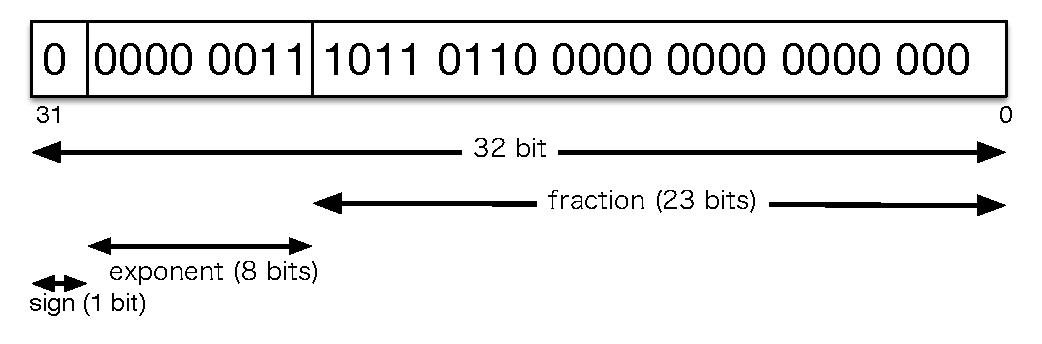
\includegraphics[scale=.4]{./Figure/elementaryCS-figFloatingPointFormat.eps}
  \end{center}
\end{frame}
\begin{frame}
\frametitle{宿題 3: 浮動小数}
  \begin{itemize}
\item 実数の浮動小数表現をやってみてください
  \end{itemize}
  \begin{block}{宿題 3}
    \begin{itemize}
\item 35.75 を浮動小数で表現してみてください
\item T2Schola に小テストがあるのでそれに答えてください
    \end{itemize}
  \end{block}
\end{frame}
\begin{frame}
\frametitle{宿題 3: 回答}
  \begin{itemize}
\item 2 進へ変換: 100011.11
\item 正規化: 1.0001111$\times 2^5$
\item 32 bit 形式に: {\scriptsize 0 0000 0101 0001 1110 0000 0000 0000 000}
    \begin{itemize}
\item 1. は省略
    \end{itemize}
\item 規格\href{http://ieeexplore.ieee.org/xpl/mostRecentIssue.jsp?punumber=2355}{\beamerbutton{IEEE 754}}では下駄 (bais) をはかせるので\(5+127=132\Rightarrow\) 1000 0100
\item 32 bit 形式に: {\scriptsize 0 1000 0100 0001 1110 0000 0000 0000 000}
  \end{itemize}
\end{frame}
\subsection{浮動小数の算術演算}
\begin{frame}[shrink,fragile]
\frametitle{浮動小数演算の変な現象 1}
  \begin{itemize}
\item roundoff.py を実行してみます
\item 結果が予測と少し違うことになります
\item \(0.6_{(10)}\) は \((0.1001\ldots)_{(2)}\), \(0.4_{(10)}\) は \((0.0110\ldots)_{(2)}\), \(0.2_{(10)}\) は \((0.0011\ldots)_{(2)}\) となります
  \end{itemize}
  \begin{lstlisting}[caption={roundoff.py},label=lst:roundoff]
if (float(0.6)-float(0.4)==float(0.2)):
   print("is equal")
else:
   print("not equal")
  \end{lstlisting}
\end{frame}
\begin{frame}[shrink,fragile]
\frametitle{浮動小数演算の変な現象 2}
  \begin{itemize}
\item machine\_epsilon.py を実行してみます
\item 結果が予測と少し違うことになります
\item この原因についてみていきます
  \end{itemize}
  \begin{lstlisting}[caption={machine\_epsilon.py},label=lst:epsilon]
# Machine epsilon
import sys

epsilon, old, prod =1.0, 0.0, 0.0
cnt=0
while (prod!=1.0):
  print(epsilon)
  old = epsilon
  cnt=cnt+1
  epsilon=epsilon/2.0
  prod=epsilon+1.0
print("Calculated machine epsilon:",old)
print("System information in Python:",sys.float_info.epsilon)
  \end{lstlisting}
\end{frame}
\begin{frame}[shrink]
\frametitle{浮動小数数の算術演算}
  \begin{itemize}
\item 正規化した 2 つの浮動小数 \(X, Y\) を \(X=F_x\times 10^{e_x}, Y=F_y\times 10^{e_y}\) とする
\item 乗算: \(XY=(F_x\times 10^{e_x})(F_y\times 10^{e_y})=F_xF_y\times 10^{e_x+e_y}\)
\item 除算: \(\frac{X}{Y}=\frac{(F_x\times 10^{e_x})}{(F_y\times 10^{e_y})}=\frac{F_x}{F_y}\times 10^{e_x-e_y}\)
\item 加算\(\cdot\)減算: \(X\pm Y=(F_x\times 10^{e_x})\pm(F_y\times 10^{e_y})=(F_x\pm F_y\cdot 10^{e_y-e_x})\times 10^{e_x}\)
    \begin{itemize}
\item ただし,\(e_x\geq e_y\)
\item \(F_y\cdot 10^{e_y-e_x}\) は指数を大きい方に揃えたときの $Y$ の仮数
    \end{itemize}
\item 演算結果も正規化するので指数は調整が必要
  \end{itemize}
  \begin{example}[算術演算の例]
    \begin{columns}[t]
      \begin{column}{4.5cm}
        \begin{math}
          \begin{array}{cll}
&0.2184&\times 10^2\\
\times&0.2512&\times 10^2\\
\hline
&0.07998208&\times 10^4\\
=&0.7998208&\times 10^3\\
          \end{array}
        \end{math}
      \end{column}
      \begin{column}{4.5cm}
        \begin{math}
          \begin{array}{cll}
&0.2844&\times 10^3\\
+&0.4162&\times 10^1\\
\hline
&0.288562&\times 10^3\\
          \end{array}
        \end{math}
      \end{column}
    \end{columns}
  \end{example}
\end{frame}
%\begin{frame}
%\frametitle{算術演算の誤差}
%  \begin{itemize}
%\item 4 桁までしか記憶できないと仮定
%\item \(0.2844\cdot 10^3+0.4162\cdot 10^1=0.288562\cdot 10^3=(0.2885+0.000062)\cdot 10^3=0.2885\cdot 10^3+0.6200\cdot 10^{-1}\)
%\item \(0.288562\)が真の値となるが \(0.2885\) までしか記憶できないので
%\item \(0.6200\cdot 10^{-1}(=0.000062\cdot 10^3)\) について調整する必要がある
%  \end{itemize}
%  \begin{example}[\(0.2844\cdot 10^3+0.4162\cdot 10^1\)]
%    \begin{columns}[t]
%      \begin{column}{4.5cm}
%        \begin{math}
%          \begin{array}{cll}
%&0.2844&\times 10^3\\
%+&0.4162&\times 10^1\\
%\hline
%&0.288562&\times 10^3\\
%          \end{array}
%        \end{math}
%      \end{column}
%      \begin{column}{4.5cm}
%        \begin{math}
%          \begin{array}{cll}
%&0.2844&\times 10^3\\
%+&0.004162&\times 10^3\\
%\hline
%&0.288562&\times 10^3\\
%          \end{array}
%        \end{math}
%      \end{column}
%    \end{columns}
%  \end{example}
%\end{frame}
\section{誤差のおはなし}
\subsection{丸め誤差 (roundoff error)}
\begin{frame}[shrink]
\frametitle{誤差とは}
  \begin{itemize}
\item コンピュータの中では実数は有限個の 0 と 1 の組み合わせ(浮動小数)で表しています
\item なので,本来あるべき真値を適当な浮動小数で近似している
\item 近似値-真値 を誤差という
  \end{itemize}
\end{frame}
\begin{frame}[shrink]
\frametitle{丸め誤差 (roundoff error)}
  \begin{itemize}
\item 表現可能な範囲に丸めることを丸め誤差という(\lstref{lst:roundoff}参照)
\item 演算結果も丸める
\item $Z$ を演算結果とする
\item $d$ 桁だけ記憶できるとして,先頭の $d$ 桁を $F$,残りを $f$ とすると,\(Z=F\cdot 10^{e_z}+f\cdot 10^{e_z-d}\)
\item $f$ の値で四捨五入することにして
    \begin{displaymath}
      \begin{array}{ll}
|f|<0.5 \mbox{のとき} & |Z|=|F|\cdot 10^{e_z-d}\\
|f|\geq 0.5 \mbox{のとき} & |Z|=|F|\cdot 10^{e_z-d}+\cdot 10^{e_z-d}
      \end{array}
    \end{displaymath}
\item 丸め誤差 $\epsilon_z$ とすれば
    \begin{displaymath}
      \begin{array}{ll}
|f|<0.5 \mbox{のとき} & |\epsilon_z|=|f|\cdot 10^{e_z-d}\\
|f|\geq 0.5 \mbox{のとき} & |\epsilon_z|=|1-f|\cdot 10^{e_z-d}
      \end{array}
    \end{displaymath}
  \end{itemize}
  \begin{example}[\(0.2844\cdot 10^3+0.4162\cdot 10^1\)]
    \begin{itemize}
\item \(0.2844\cdot 10^3+0.4162\cdot 10^1=0.2885\cdot 10^3+0.6200\cdot 10^{-1}\)
\item \(|Z|=0.2885\cdot 10^3+10^{3-4}=0.2886\cdot 10^3\)
\item \(|\epsilon_z|=|1-0.6200|\cdot 10^{3-4}=0.48\cdot 10^{-1}\)
    \end{itemize}
  \end{example}
\end{frame}
%\begin{frame}
%\frametitle{相対誤差 (relative error)}
%  \begin{itemize}
%\item 計算のコストだけでなくときには計算精度も重要になる
%\item 真の値 $x^t$,観測した値 $x$ として誤差 \(\epsilon_x=x^t-x\)
%\item \(|\epsilon_x|=|x^t-x|\) を絶対誤差という
%\item 相対誤差 \(r_x=\frac{\epsilon_{x}}{x}=\frac{x^t-x}{x}\) で精度を測る
%  \end{itemize}
%  \begin{example}[相対誤差の例]
%    \begin{itemize}
%\item \(x_t=9, x=10\) と \(y_t=999, y=1000\) の場合を考える
%\item $x$ と $y$ の誤差はどちらも \(-1\)
%\item $x$ と $y$ の相対誤差はそれぞれ \(r_x=\frac{-1}{10}, r_y=\frac{-1}{1000}\)
%    \end{itemize}
%  \end{example}
%\end{frame}
%\subsection{誤差の伝搬 (propagation of errors)}
%\begin{frame}
%\frametitle{誤差の伝搬 (propagation of errors)}
%  \begin{itemize}
%\item 誤差は計算中伝播して計算結果を不正確にしてしまう
%\item 算術式中の誤差がどう蓄積されていくかをみる
%\item ある数 $x, y$ としてそれぞれが誤差 \(\epsilon_x, \epsilon_y\) を持つとする
%\item このときの演算 \(x\oplus y\) の誤差 \(\epsilon_{x\oplus y}\) は
%    \begin{displaymath}
%\epsilon_{x\oplus y}=(x^t\oplus y^t)-(x\oplus y)
%    \end{displaymath}
%\item \(x^t\oplus y^t\) は真の演算結果で, \(x\oplus y\) は実際の結果
%\item 先の誤差の定義からこれが導ける
%  \end{itemize}
%\end{frame}
%\begin{frame}[shrink]
%\frametitle{誤差公式}
%  \begin{itemize}
%\item 各演算についてつぎの関係が成り立つ
%  \end{itemize}
%  \begin{theorem}[誤差公式]
%    \begin{math}
%      \begin{array}{lclclclcl}
%\scriptsize
%\epsilon_{x+y}&=&(x^t+y^t)-(x+y)&=&(x^t-x)+(y^t-y)&=&\epsilon_x+\epsilon_y\\
%\epsilon_{x-y}&=&(x^t-y^t)-(x-y)&=&(x^t-x)-(y^t-y)&=&\epsilon_x-\epsilon_y\\
%      \end{array}
%    \end{math}
%    \begin{math}
%      \begin{array}{lclclclcl}
%\epsilon_{xy}&=&(x^ty^t)-(xy)&=&(x+\epsilon_x)(y+\epsilon_y)-(xy)&=&\epsilon_x y+\epsilon_y x\\
%      \end{array}
%    \end{math}
%    \begin{math}
%      \begin{array}{lclclclcl}
%\epsilon_{\frac{x}{y}}&=&\frac{x^t}{y^t}-\frac{x}{y}&=&\frac{x^ty-y^tx}{y^ty}&=&\frac{(x+\epsilon_x)y-(y+\epsilon_y)x}{(y+\epsilon_y)y}\\
%&=&\frac{xy+\epsilon_xy-xy+x\epsilon_y}{y^2(1+\frac{\epsilon_y}{y})}&=&\frac{\epsilon_xy-\epsilon_yx}{y^2}\\
%      \end{array}
%    \end{math}
%    \begin{itemize}
%\item \(\epsilon_x\epsilon_y\) は十分小さいとして無視
%\item \(|\frac{\epsilon_y}{y}|\) は \(|\frac{\epsilon_y}{y}|\ll 1\) のとき無視
%\item これに各演算の丸め誤差 \(\alpha\) を加えたて誤差公式とする
%      \begin{itemize}
%\item たとえば 4 桁までしか記憶できないのであれば演算結果も 4 桁に丸められる
%      \end{itemize}
%    \end{itemize}
%  \end{theorem}
%\end{frame}
%\begin{frame}[shrink]
%\frametitle{相対誤差公式}
%  \begin{itemize}
%\item 相対誤差公式を導く
%\item 先の相対誤差の定義より
%    \begin{displaymath}
%r_{x\oplus y}=\frac{\epsilon_{x\oplus y}}{x\oplus y}
%    \end{displaymath}
%\item とすれば誤差公式よりつぎの相対誤差公式をえる
%  \end{itemize}
%  \begin{theorem}[相対誤差公式]
%    \begin{math}
%      \begin{array}{rclcl}
%r_{x+y}&=&\frac{\epsilon_x+\epsilon_y}{x+y}+\alpha&=&r_x\frac{x}{x+y}+r_y\frac{y}{x+y}+\alpha\\
%r_{x-y}&=&\frac{\epsilon_x-\epsilon_y}{x-y}+\alpha&=&r_x\frac{x}{x-y}+r_y\frac{-y}{x-y}+\alpha\\
%r_{xy}&=&\frac{\epsilon_x y+\epsilon_y x}{xy}+\alpha&=&r_x\ 1+r_y\ 1+\alpha\\
%r_{xy}&=&\frac{\frac{\epsilon_x y-\epsilon_y x}{y^2}}{\frac{x}{y}}+\alpha&=&r_x\ 1+r_y\ (-1)+\alpha
%      \end{array}
%    \end{math}
%  \end{theorem}
%\end{frame}
%\begin{frame}[shrink]
%\frametitle{誤差伝播の解析}
%  \begin{itemize}
%\item 相対誤差公式を使って誤差伝播の解析を行う
%  \end{itemize}
%  \begin{example}[和における誤差伝播]
%    \begin{itemize}
%\item \(r_0, r_1, r_2, r_3\) を実数 \(a_0,a_1,a_2,a_3\) の相対誤差とする
%\item \(S=(((a_0+a_1)+a_2)+a_3)\) の相対誤差を求める
%    \end{itemize}
%  \end{example}
%\end{frame}
\subsection{情報落ち誤差}
\begin{frame}[shrink]
\frametitle{情報落ち誤差(loss of trailing digits)}
  \begin{itemize}
\item 絶対値が大きく異なる 2 つの数の加減算では小さい数が無視されることがある
\item \lstref{lst:epsilon} で見たような場合
  \end{itemize}
\end{frame}
\subsection{打ち切り誤差 (truncation error)}
\begin{frame}[shrink]\label{sl:back}
\frametitle{打ち切り誤差 (truncation error)}
  \begin{itemize}
\item コンピュータでは無限に繰り返して値をもとめることはできない
\item 有限回の計算で値を計算し,それを求める値の近似値としてもちいる
\item このときの誤差を打切り誤差という
  \end{itemize}
  \begin{example}[\(\sin(x)\)のマクローリン展開]
    \begin{itemize}
\item \(sin(x)=x-\frac{x^3}{3!}+\frac{x^5}{5!}-\frac{x^7}{7!}+\cdots+(-1)^{n}\frac{x^{2n+1}}{(2n+1)!}+\cdots\)
\item gnuplot で試してみてください
    \end{itemize}
  \end{example}
  \begin{example}[平方根の計算]
    \begin{itemize}
%\item \href{run:newton.command}{\beamerbutton{ニュートン法}}
\item newton.py を参照\hyperlink{newton-is_enough-rec}{\beamerbutton{プログラム例}}
\item \(\sqrt{a}\) を求めてみる
\item \(f(x)=x^2-a\) として \(f(x)=0\) となる $x$ を求める
\item \(k+1\) 番目の近似値 \(x_{k+1}\) を
      \begin{displaymath}
x_{k+1} = x_k-\frac{f(x_k)}{f'(x_k)} = \frac{1}{2}(x_k+\frac{a}{x_k})
      \end{displaymath}
    \end{itemize}
  \end{example}
\end{frame}
%\section{まとめ}
%\begin{frame}[shrink,fragile]
%\frametitle{数値計算}
%  \begin{itemize}
%\item ここで取り上げたおはなしは数値計算(計算機科学の一分野)のなかの計算誤差をとりあげたもの
%\item シミュレーションなどではある関数の実際の数値を必要とする場合がある
%    \begin{itemize}
%\item 例えば,方程式 \(f(x)=0\) の $x$ を数値的に求める
%    \end{itemize}
%\item 数値計算の手順
%    \begin{itemize}
%\item 最初に適当な 1 次近似 \(x_0\) を選んで,
%\item より良い近似を求め,
%\item 適当な収束条件を満たすまで繰り返す (マシンイプシロンは収束条件の重要な指標)
%    \end{itemize}
%\item \(f\) は複雑なので数値的な解を求めるいろいろな算法を考察
%  \end{itemize}
%\end{frame}

%
%%% STRINGS
%
%\subsection{文字データ}
%\begin{frame}
%\frametitle{文字データの表現}
%  \begin{itemize}
%\item コンピュータは数値だけでなく文字も処理することができる
%\item 文字をコード化して処理する
%\item 詳細は第 3 回目で
%  \end{itemize}
%\end{frame}
%
%%% SOUND and MOVIE
%
%\subsection{画像と音}
%\begin{frame}
%\frametitle{画像}
%  \begin{itemize}
%\item つぎは画像データについて見てみます
%\item 画像も二進列で表せます
%\item ビットマップというファイル形式
%    \begin{itemize}
%\item マス目にわけ,白い部分を 1 ,黒い部分を 0 としてビットの列を作る
%    \end{itemize}
%  \end{itemize}
%\centering
%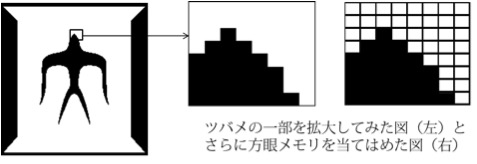
\includegraphics[scale=0.4]{./Figure/TITECH-logo.jpg}
%\end{frame}
%\begin{frame}
%\frametitle{音}
%  \begin{itemize}
%\item つぎは音データ
%\item 波の符号化
%    \begin{itemize}
%\item (a) は波形
%\item (b) は標本化
%\item (c) はそれぞれの標本値
%\item この標本値を順番にならべた二進列
%    \end{itemize}
%\item 音符の符号化 (Standard MIDI)
%    \begin{itemize}
%\item 音符やテンポを符号化
%\item \movie[once,externalviewer]{\beamerbutton{.mid}}{./Figure/Nodame.mid}
%    \end{itemize}
%  \end{itemize}
%  \begin{center}
%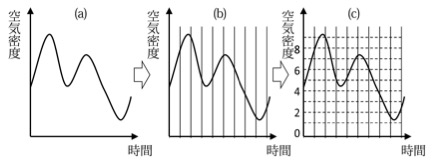
\includegraphics[scale=0.4]{./Figure/wave.jpg}
%  \end{center}
%\end{frame}
%
%%% COMPUTER
%
%\section{コンピュータの中では}
%\begin{frame}
%\frametitle{コンピュータの中では}
%  \begin{itemize}
%\item コンピュータの命令自体も符号化されてます
%\item CPU (Central Processing Unit) ごとに命令セットも符号も異なっています
%\item ここでは CPU が命令を実行するサイクルについて見てみます
%  \end{itemize}
%  \begin{center}
%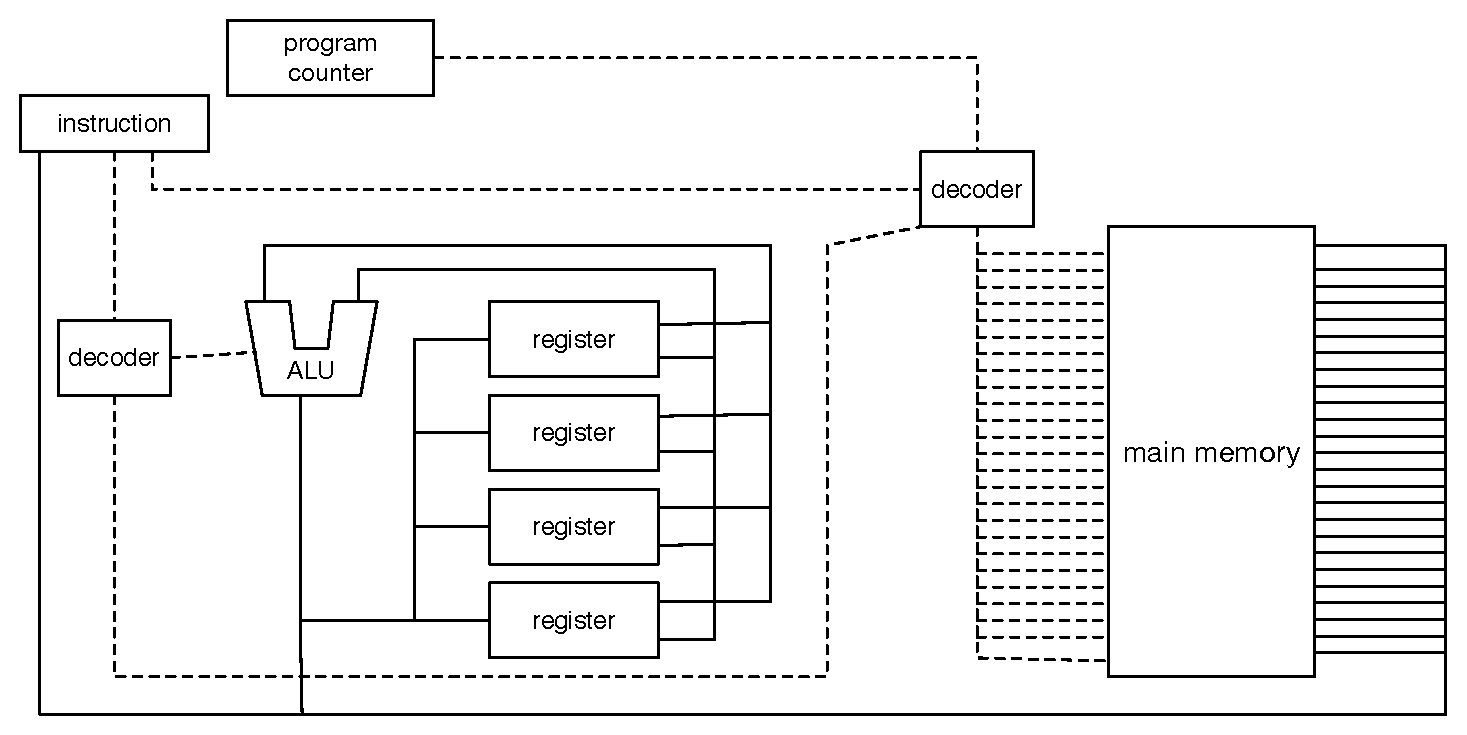
\includegraphics[scale=0.4]{./Figure/elementaryCS-figCPU}
%  \end{center}
%\end{frame}
%\begin{frame}
%\frametitle{演算のサイクル}
%  \begin{enumerate}
%\scriptsize
%\item instruction に命令をフェッチ
%\item メインメモリからレジスタにデータを移動
%\item ALU (Arithmetic and Logic Unit) がレジスタからデータを取り出す
%\item ALU で演算
%\item 結果をレジスタに書き込む
%\item レジスタからメインメモリにデータを移動
%\item ADD cx dx bx という命令を例にすると下図のようになります
%  \end{enumerate}
%  \begin{center}
%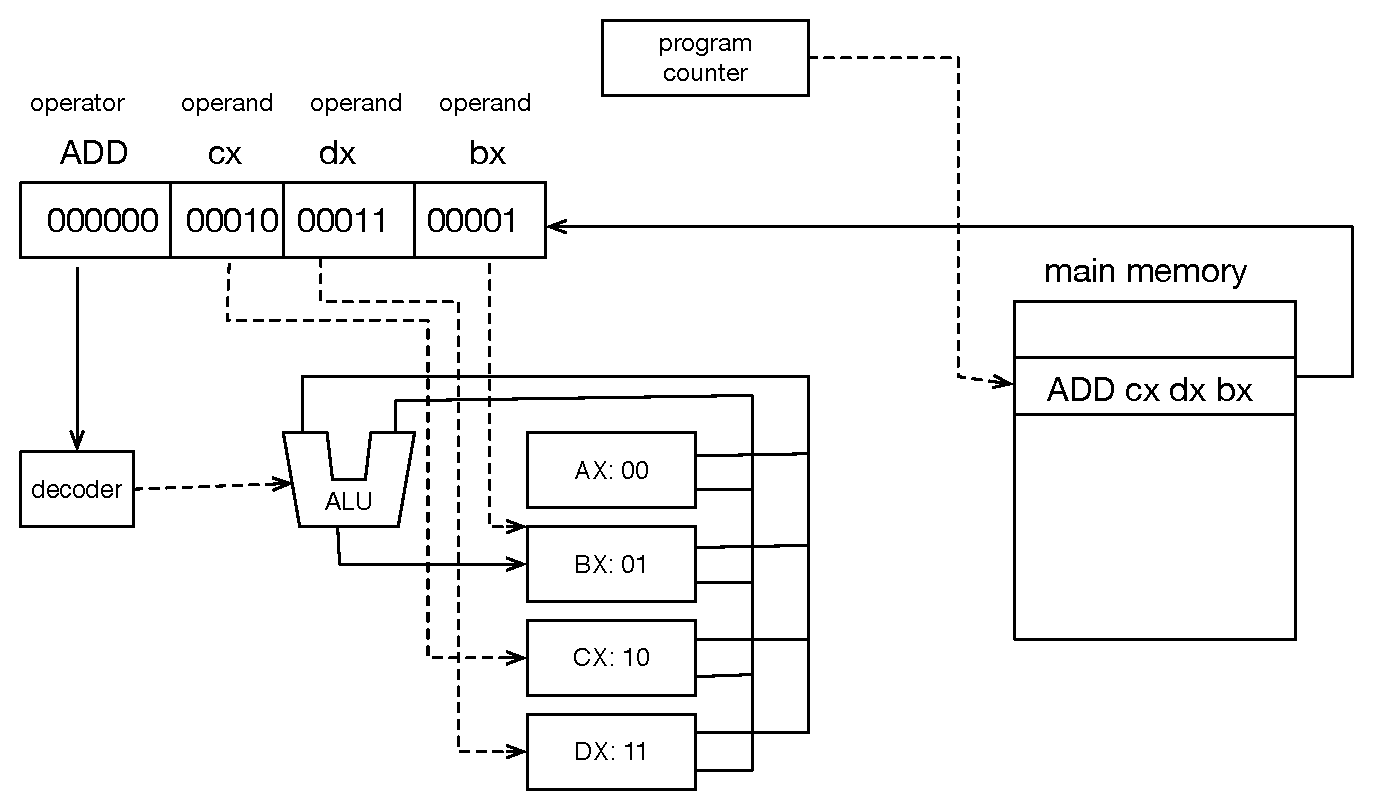
\includegraphics[scale=0.3]{./Figure/elementaryCS-figCycle}
%  \end{center}
%\end{frame}
\section{計算 = \(\pm 1\) と繰り返し}
\subsection{計算とは}
\begin{frame}
\frametitle{計算とは}
  \begin{itemize}
\item つぎは計算について
\item 計算には入力と出力があって
\item 入力と出力の関係をとくに関数とよぶ
\item この場合,ある入力に対して出力は一意に決まる
\item また関数には適当な名前をつけることができる
\item 関数を合成してより複雑な計算を実現していく
\item ここまではまだ入出力の関係としか云っていない
  \end{itemize}
  \begin{example}[最大公約数]
最大公約数 \(gcd(n,m)\) は \(n, m\) の公約数で最大ものと定義されるが,どう求めるか方法は書いていない
  \end{example}
\end{frame}
\begin{frame}[fragile,shrink]
\frametitle{計算の方法}
  \begin{itemize}
\item 計算の方法について考える
\item 計算機科学では関数といった時はこちらの意味
\item 計算の方法のことをアルゴリズム (algorithm) といっている
\item アルゴリズムとデータを特定の形式で書いたものがプログラム
  \end{itemize}
  \begin{lstlisting}[caption={最大公約数},label=gcd]
# Greatest common divisor
# Input: 自然数 x, y
# Output: gcd(x,y)
###

def gcd(x,y):
  ans=1
  n=min(x,y)
  for i in range(1,n):
    if (x%i==0) and (y%i==0):
      ans=i
  return (ans)
print(gcd(x,y))
  \end{lstlisting}
\hfill{\hyperlink{if}{\beamerbutton{Back to if-slide}}}
\end{frame}
\subsection{計算の基本要素}
\begin{frame}[fragile]
\frametitle{計算の基本要素}
\framesubtitle{計算 = \(\pm 1\) と繰り返し}
  \begin{itemize}
\item 合成していくとして最も基本となるものは何か
\item 結論から云ってしまえば,ある値に $\pm 1$ する操作と繰り返しと条件分岐である
  \end{itemize}
  \begin{lstlisting}[caption={加算},label=add]
# add.py
# Input: 自然数 a, b
# Output: a + b
###

a = int(input("? "))  # 入力された自然数を a に代入
b = int(input("? "))  # 入力された自然数を b に代入
wa = a                # a の値を wa に代入
while b > 0:          # b が 0 より大きい間は end までを繰り返す
  wa = wa + 1         #   wa + 1 の値を wa に代入
  b = b - 1           #   b - 1 の値を b に代入
print(wa)             # wa の値を出力
  \end{lstlisting}
\end{frame}
\begin{frame}[fragile,label=mult,shrink]
\frametitle{基本要素だけの乗算}
  \begin{lstlisting}[caption={乗算},label=lst:mult]
# mult_basiconly.py
# Input: 自然数 x, y
# Output: x * y
###

x = int(input("x? "))       # 入力された自然数を x に代入
y = int(input("y? "))       # 入力された自然数を y に代入
seki = 0                    # seki を 0 で初期化
while y > 0:                # y が 0 より大きい間は end までを繰り返す
  a = seki
  b = x
  wa = a                    # 和のプログラム add.py を挿入
  while b > 0:
    wa = wa + 1
    b = b - 1
  seki = wa                 # wa の値 (seki + x) を seki に代入
  y = y - 1                 # y - 1 の値を y に代入
print(seki)                 # seki の値を出力
  \end{lstlisting}
\hfill{\hyperlink{composit}{\beamerbutton{Back to composit-slide}} \hyperlink{while}{\beamerbutton{Back to while-slide}}}
\end{frame}
\section{プログラムの書き方}
\subsection{プログラミングのための仕掛け}
\begin{frame}[fragile]
\frametitle{プログラミングのための仕掛け}
  \begin{itemize}
\item プログラミング言語にはプログラミングのための 3 つの仕掛けがある
    \begin{itemize}
\item 基本式: プログラミングに関わる最も単純なもの
\item 組合せ法: 単純なものからより複雑なものをつくる (構文として定義されている)
\item 抽象化法: 合成物に名前をつけ基本式と同様に扱う
    \end{itemize}
\item データについても同様
  \end{itemize}
\end{frame}
\begin{frame}[fragile]
\frametitle{Python における基本式}
  \begin{itemize}
\item 式の基本要素は 自然数,整数,実数などがある
    \begin{itemize}
\item 自然数の例: \(286, 386, 486\) 
\item 講義では自然数だけあつかうので注意
    \end{itemize}
\item 基本要素と演算子 \(+, -, *, \slash\slash, \%, **\) などを組み合わせて式をつくる
    \begin{itemize}
\item 自然数の例: \(286+386, 486\) 
\item 入れ子にできます: \(286+(386+486)\) 
    \end{itemize}
\item 式には名前をつけることができ,この名前のことを変数と呼でいます
\item その名前で参照することもできます
    \begin{itemize}
\item 例: \(\mbox{abc}=286+386\) 
\item 例: \(\mbox{efg}=\mbox{abc}+486\) 
    \end{itemize}
\item $=$ は論理記号ではなくて代入をあらわすので注意
\item abc は \(\mbox{a}\times\mbox{b}\times\mbox{c}\) ではなく変数名なので注意
  \end{itemize}
\end{frame}
%\begin{frame}[fragile]
%\frametitle{Ruby における論理演算子}
% \begin{center}
%  \begin{tabular}{c|c|c}
%算術演算子&使用例&意味\\\hline
%+& x $+$ y & x と y の足し算\\
%-& x $-$ y & x と y の引き算\\
%*& x $*$ y & x と y のかけ算\\
%$\slash$& x $\slash$ y & x を y 割った商\\
%\%& x $\%$ y & x を y 割ったあまり\\
%**& x $**$ y & x の y 乗\\\hline
%論理演算子&使用例&意味\\\hline
%==& x == y & x と y が等しいなら真\\
%!=& x != y & x と y が等しくないなら真\\
%>=& x >= y & x は y 以上なら真\\
%<=& x <= y & x は y 以下なら真\\
%>& x > y & x は y より大きいなら真\\
%<& x < y & x は y より小さいなら真\\
%  \end{tabular}
% \end{center}
%\end{frame}
%\begin{frame}[fragile]
%\frametitle{論理の合成}
% \begin{center}
%  \begin{tabular}{c|c|c}
%論理演算子&使用例&意味\\\hline
%\&\& & p \&\& q & 論理積: 両方が真なら真\\
%$\|$ & p $\|$ q & 論理和: いずれかが真なら真\\
%! & ! p & p の否定\\
%  \end{tabular}
% \end{center}
%\end{frame}
\begin{frame}[label=composit]
\frametitle{Python における合成}
  \begin{itemize}
\item 式を順番に並べる
\item 実行は上から下へ,左から右に順番に実行される
\item 前に実行された式の結果は変数をもちいて参照
\item 実行順序を変えたいときは while や if を使う
\item \hyperlink{mult}{\beamerbutton{Jump to an example}}
  \end{itemize}
\end{frame}
\begin{frame}[fragile,label=if]
\frametitle{if 文}
  \begin{itemize}
\item 条件によって実行順序を変更する
\item \hyperlink{gcd}{\beamerbutton{Jump to an example}}
\item 条件式は \href{https://docs.python.org/ja/3/reference/expressions.html#comparisons}{\beamerbutton{Python ドキュメント 6.10, 6.11, 6.12 節}}参照
  \end{itemize}
\end{frame}
\begin{frame}[fragile,label=while]
\frametitle{while 文}
  \begin{itemize}
\item 実行列を繰り返し実行する
\item \hyperlink{mult}{\beamerbutton{Jump to an example}}
  \end{itemize}
\end{frame}
%%%
% Homework 1
%%%
\subsection{宿題 1 を動かしてみる}
\begin{frame}[fragile,shrink]
\frametitle{宿題 1 を動かしてみる}
\framesubtitle{宿題 1 \textendash $\pm 1$だけで四則演算を作る}
  \begin{itemize}
\item \href{https://sites.google.com/a/presystems.xyz/sample/home/elementary-computer-science}{\beamerbutton{https://sites.google.com/a/presystems.xyz/sample/home/elementary-computer-science}} に div-skeleton.py と sub-skeleton.py があるはずなのでそれを完成させて実行する
\item OCW-i から提出
\item ファイル名に日本語文字は使用しないでください
  \end{itemize}
  \begin{columns}
    \begin{column}{0.45\textwidth}
      \begin{lstlisting}[caption={sub.py},label=lst:sub]
# sub.py
# Input: 自然数 a, b
# Output: a - b

a = int(input("a? "))
b = int(input("b? "))
sa = a               
while    :
  sa = 
  b = 
print(sa)
      \end{lstlisting}
    \end{column}
    \begin{column}{0.45\textwidth}
      \begin{lstlisting}[caption={div.py},label=lst:div]
# div.py
# Input: 自然数 x, y
# Output: x ÷ y の商と余り

x = int(input("x? "))
y = int(input("y? "))
shou = 
amari = 
while    :
  shou = 
  amari = amari - y
print(shou)
print(amari)
      \end{lstlisting}
    \end{column}
  \end{columns}
\end{frame}
%
%%% PROGRAMMING ENVIRONMENT
%
\section{開発環境構築}
\subsection{Python3 環境構築}
\begin{frame}[shrink]
\frametitle{環境構築}
\framesubtitle{Python3}
  \begin{itemize}
\item Python を利用するためには各自の PC 上に環境を構築する必要があります
\item すでに python 開発環境を持っている人は以下の作業は不要です
\item 各状況に合わせて環境を作っていきます
    \begin{itemize}
\item Cloud で利用したい方は\href{https://www.pythonanywhere.com/}{\beamerbutton{https://www.pythonanywhere.com/}}で beginner account を作成(無料でインストール不要です)
\item Windows, Mac OSX, Linux で自分の PC に環境を作りたい方は\href{https://www.python.jp/install/install.html}{\beamerbutton{https://www.python.jp/}}を参照
    \end{itemize}
  \end{itemize}
\end{frame}
\begin{frame}[shrink,containsverbatim]
\frametitle{Pythonanywhere のアカウント開設}
  \begin{itemize}
\item ``Start running Python on line in less than a minute'' をクリック
  \end{itemize}
\includegraphics[width=1\textwidth]{../InformationLiteracy/Figure/IL-figStartAnywhere.jpg}
\end{frame}
\begin{frame}[shrink,containsverbatim]
\frametitle{Pythonanywhere のアカウント作成}
  \begin{itemize}
\item ``Create a Biginner account'' をクリック
\item 無料のアカウントを作成します
  \end{itemize}
\includegraphics[width=1\textwidth]{../InformationLiteracy/Figure/IL-figCreateAnywhereAccount.jpg}
\end{frame}
\begin{frame}[shrink,containsverbatim]
\frametitle{Pythonanywhere のアカウント登録}
  \begin{itemize}
\item ``Username'' を入力(任意)
\item ``Email'' を入力(m ドメイン以外でもかまいません)
\item ``Password'' を入力
\item ``I agree$\ldots$'' にチェック
\item ``Register'' をクリック
  \end{itemize}
\includegraphics[width=1\textwidth]{../InformationLiteracy/Figure/IL-figAnywhereRegister.jpg}
\end{frame}
\begin{frame}[shrink,containsverbatim]
\frametitle{登録後の画面}
  \begin{itemize}
\item 登録アドレスにメイルが届くので確認
\item 以下のような画面が見えれば OK
  \end{itemize}
  \begin{itembox}{登録後の画面}
\includegraphics[width=1\textwidth]{../InformationLiteracy/Figure/IL-figAnywhereDashboard.jpg}
  \end{itembox}
\end{frame}
\begin{frame}[shrink,containsverbatim]
\frametitle{自身の PC 上にインストールひと}
  \begin{itemize}
\item Idle を起動してください
  \end{itemize}
  \begin{columns}[t]
    \begin{column}{0.5\textwidth}
      \begin{itembox}{\footnotesize Mac, Linux のひと}
        \begin{itemize}
\scriptsize
\item ターミナルを起動して idle3 と入力
        \end{itemize}
        \begin{verbatim}
> idle3
        \end{verbatim}
      \end{itembox}
    \end{column}
    \begin{column}{0.5\textwidth}
      \begin{itembox}{\footnotesize Windows のひと}
        \begin{itemize}
\item スタートメニューから IDLE を起動
        \end{itemize}
      \end{itembox}
    \end{column}
  \end{columns}
\end{frame}
\begin{frame}[shrink,containsverbatim]
\frametitle{開発統合環境}
\framesubtitle{IDLE と Pythonanywhere}
  \begin{itemize}
\item Mac, Windows, Linux の人もこれで準備ができました
\item それぞれ以下のような画面が見えるはずです
\item 以後,いずれかの開発統合環境を利用していきます
\item Pythonanywhere や IDLE は編集,実行が統合された環境を提供しています
\item IDLE の使い方は\href{https://docs.python.org/ja/3/library/idle.html?highlight=idle}{\beamerbutton{Python 公式}}を参照
    \begin{itemize}
\item \href{http://www.isc.meiji.ac.jp/~mizutani/python/intro1_python.html}{\beamerbutton{http://www.isc.meiji.ac.jp/~mizutani/python/intro1\_python.html}}も参考になるかも
    \end{itemize}
  \end{itemize}
  \begin{columns}[c]
    \begin{column}{5cm}
\includegraphics[width=1\textwidth]{../InformationLiteracy/Figure/IL-figIDLE.jpg}
    \end{column}
    \begin{column}{5cm}
\includegraphics[width=1\textwidth]{../InformationLiteracy/Figure/IL-figPythonanywhere.jpg}
    \end{column}
  \end{columns}
\end{frame}
\subsection{動作確認}
\begin{frame}[shrink,containsverbatim]
\frametitle{開発環境テスト用コード}
%\vspace{-2zw}
%  \begin{lstlisting}[caption={環境テスト用コード},label=lst:test,numbers=none]
%import matplotlib.pyplot as plt
%print('Hello World')
%plt.plot([1, 2, 3, 4])
%plt.show()
%  \end{lstlisting}
  \begin{itemize}
\item \href{https://sites.google.com/presystems.xyz/elementarycs/top}{\beamerbutton{https://sites.google.com/presystems.xyz/elementarycs/top}} 
からhello.pyをダウンロード
  \end{itemize}
\vspace{-1em}
  \begin{columns}[t]
    \begin{column}{0.5\textwidth}
      \begin{itembox}{\footnotesize IDLE 利用のひと}
        \begin{itemize}
\scriptsize
\item File->Open で hello.py を開く
        \end{itemize}
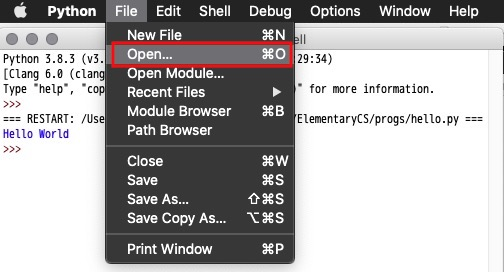
\includegraphics[width=1\textwidth]{./Figure/elementaryCS-figOpenFile.jpg}
      \end{itembox}
    \end{column}
    \begin{column}{0.5\textwidth}
      \begin{itembox}{\footnotesize Pythonanywhere 利用のひと}
\scriptsize
        \begin{itemize}
\item 右上 ``Files'' をクリック
\item ''upload'' をクリックして hello.py をアップロード
\item hello.py をクリックすると中が見れます
        \end{itemize}
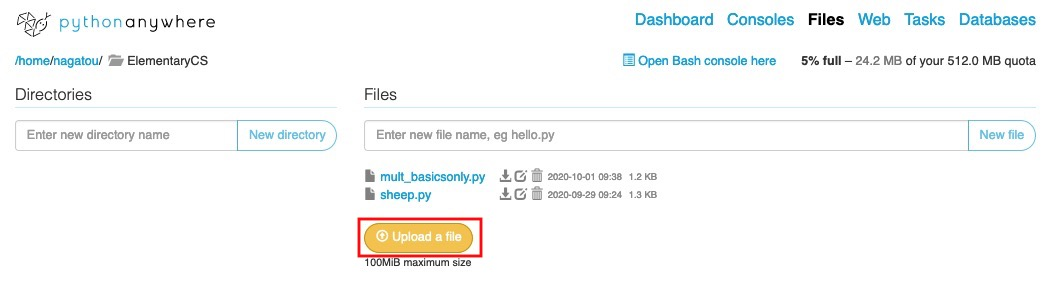
\includegraphics[width=1\textwidth]{./Figure/elementaryCS-figUpload.jpg}
      \end{itembox}
    \end{column}
  \end{columns}
\end{frame}
\begin{frame}[shrink,containsverbatim]
\frametitle{プログラムの実行}
%  \begin{itemize}
%\item \href{https://sites.google.com/a/presystems.xyz/sample/home/information-literacy}{\beamerbutton{https://sites.google.com/a/presystems.xyz/sample/home/information-literacy}}から test.py をダウンロード
%  \end{itemize}
  \begin{columns}[t]
    \begin{column}{0.5\textwidth}
      \begin{itembox}{\footnotesize IDLE 利用のひと}
        \begin{itemize}
\scriptsize
\item Run->Run Module をクリック
\item ``Hello World'' が表示されれば正常
        \end{itemize}
\includegraphics[width=1\textwidth]{../InformationLiteracy/Figure/IL-figTestIDLE.jpg}
      \end{itembox}
    \end{column}
    \begin{column}{0.5\textwidth}
      \begin{itembox}{\footnotesize Pythonanywhere 利用のひと}
\scriptsize
        \begin{itemize}
\item Run this file をクリック
\item 下半分の黒い画面に ``Hello World'' と表示されれば正常
\item 下半分の黒い画面で exit() と入力してください
        \end{itemize}
\includegraphics[width=1\textwidth]{../InformationLiteracy/Figure/IL-figTestCloud.jpg}
      \end{itembox}
    \end{column}
  \end{columns}
\end{frame}

